\section{软件工程}
软件工程是一门研究用工程化的方法构建和维护有效的、实用的和高质量的软件的学科

软件工程的两大视角
\vspace{-0.8em}
\begin{multicols}{2}
    \begin{itemize}
        \item 管理视角:能否复制成功
        \item 技术视角:是否可以将问题解决得更好
    \end{itemize}
\end{multicols}
\vspace{-1em}


\subsection{管理}
\begin{itemize}
    \item 管理的三大关键要素:目标、状态(是在接近目标还是在远离目标)和纠偏
    \item 大部分情况下,管理仅仅是试图复制其他地方(场景)的成功,但是这种复制一般不容易
    \item 软件项目管理是为了降低/减少各种无谓的损耗来实现本该有的性能
    \item 软件过程改进是为了达到更好的效能,其中质量/缺陷是首要目标或限制
\end{itemize}

\subsubsection{软件项目管理}
\begin{itemize}
    \item 典型的三大目标:成本、质量和工期
    \item 定义:软件项目管理是应用方法、工具、技术以及人员能力来完成软件项目,实现项目目标的过程
    \begin{itemize}
        \item 软件项目管理包括估算、计划、跟踪、风险管理、范围管理、人员管理、沟通管理等等
        \item 软件项目管理的对象是各类软件项目
    \end{itemize}
    \item 可以细分为两种管理视角:软件过程与生命周期模型
\end{itemize}

\subsubsection{软件过程管理}
\begin{itemize}
    \item 软件过程管理的对象是软件过程
    \item 软件过程管理的目的是为了让软件过程在开发效率、质量等方面有着更好性能绩效(Performance)
\end{itemize}

\subsubsection{软件过程管理与软件过程改进}
\vspace{-0.8em}
\begin{multicols}{2}
    \begin{itemize}
        \item 两者含义接近
        \item 软件过程管理参考模型 CMM/CMMI, SPICE 等
        \item 软件过程改进参考元模型 PDCA, IDEAL等
    \end{itemize}
\end{multicols}
\vspace{-1em}


\subsubsection{考试题目}
\begin{problem}
    下列哪些项不属于管理活动应该包含的要素?
	\uline{ABD}    
    \vspace{-0.8em}
    \begin{multicols}{4}
        \begin{enumerate}[label=\Alph*.]
            \item 成本
            \item 质量
            \item 目标
            \item 工期
        \end{enumerate}
    \end{multicols}
    \vspace{-1em}
\end{problem}

\begin{problem}
软件项目管理和软件过程管理
\begin{itemize}
    \item 软件项目管理是应用方法、工具、技术以及人员能力来完成软件项目,实现项目目标的过程
    \item 软件过程管理是为了让软件过程在开发效率、质量等方面有着更好性能绩效
\end{itemize}
\end{problem}


\subsection{软件过程}
软件过程是为了实现一个或者多个事先定义的目标而建立起来的一组实践的集合。这一组实践往往有一定的先后顺序,作为一个整体来实现事先定义的一个或者多个目标。

\subsubsection{广义软件过程}
\begin{itemize}
    \item 理论基石:软件产品和服务的质量,很大程度上取决于生产和维护该软件或者服务的过程的质量
    \item 包括:技术、人员以及狭义过程
    \item 同义词:软件开发方法、软件开发过程
    \begin{itemize}
        \item 净室Clean Room方法、极限编程方法、Scrum方法、Gate方法
        \begin{itemize}
            \item Clean Room工程过程和 CMM 管理过程互为补充
            \item Clean Room比 CMM 更注重质量,更偏向于使用一些数学工具
        \end{itemize}
        \item 更一般的,敏捷软件过程/方法、轻量型过程/方法及重型过程/方法等描述也是恰当的
    \end{itemize}
\end{itemize}

\subsubsection{生命周期模型}
\begin{itemize}
    \item 生命周期模型是对软件过程的一种人为划分
    \item 典型生命周期模型:瀑布模型、迭代式模型、增量模型、螺旋模型、原型法等等
\end{itemize}

\subsubsection{考试题目}
\begin{problem}
生命周期模型与软件过程的区别和联系
\begin{enumerate}[label=\arabic*.]
    \item 生命周期模型是对一个软件开发过程的人为划分
    \item 生命周期模型是软件开发过程的框架,是对软件开发过程的一种粗粒度划分
    \item 生命周期模型往往不包括技术实践
\end{enumerate}
\end{problem}

\begin{problem}
我们如何理解瀑布模型
\begin{enumerate}[label=\arabic*.]
    \item 瀑布模型不是单一模型,是一系列模型,覆盖最简单场景(过程元素少)到最复杂的场景(过程元素多)
    \item 软件项目应该结合实际情况选择合适过程元素的瀑布模型,基本原则是,项目面临困难和挑战越多,选择的模型应该越复杂
    \item 软件项目团队往往低估项目的挑战,选择了过于简单的不适用的瀑布模型
\end{enumerate} 
\end{problem}

\begin{problem}
	下列名词和术语中不属于软件过程的有哪些?
	\uline{BD}    
    \vspace{-0.8em}
    \begin{multicols}{4}
        \begin{enumerate}[label=\Alph*.]
            \item SCRUM
            \item CMM/CMMI
            \item GATE 方法
            \item IDEAL
        \end{enumerate}
    \end{multicols}
    \vspace{-1em}
\end{problem}

\begin{problem}
{\kaishu 软件过程管理是软件项目管理应该要实现目标:}软件过程管理和软件项目管理完全是两回事,项目过程管理应当有专门的人去做。因此并不是实现目标,错误的。
\end{problem}

\begin{problem}
{\kaishu 在公司导入敏捷过程是我们今年过程改进的主要目标:}过程管理和过程改进是类似的,这个说法在概念上是合适的,但是操作的时候可能存在问题。
\end{problem}

\begin{problem}
{\kaishu XP与CMM/CMMI是对立的两种软件开发方法:}CMM和CMMI并不是软件开发方法,而是软件过程管理和改进,CMM和CMMI是没有较大区别的,错误的。XP的观念确实与严格的CMM/CMMI是对立的,XP是软件开发方法,敏捷的。
\end{problem}

\begin{problem}
{\kaishu CMM/CMMI不适合当今互联网环境的项目管理需求:}CMM/CMMI是用来做过程管理和改进的,根本不是满足项目管理需求的手段,正确的。
\end{problem}

\begin{problem}
{\kaishu PDCA和IDEAL不适合在敏捷环境中使用:}PDCA,IDEAL是软件过程改进参考元模型,因此是适合在敏捷环境中使用的,错误的。
\end{problem}

\begin{problem}
{\kaishu 不同的软件开发过程应该使用不同的生命周期模型,反之亦如此:}生命周期模型是由人类划分的,不一定,错误的,
\end{problem}



\subsection{软件过程管理/改进模型:CMM}
定义:CMM是一种用于评价软件承包能力并帮助其改善软件质量的方法,侧重于软件开发过程的管理及工程能力的提高与评估。

级别:分五个级别,一级为初始级,二级为可重复级,三级为已定义级,四级为已管理级,五级为优化级
\begin{enumerate}[label=\arabic*.]
    \item 初始级 Initial:处于该级别的组织基本上没有健全的软件工程管理制度。要精确地预测产品的开发实践和费用之类重要的项目,是不可能的。
    \begin{itemize}
        \item 每件事情都用特殊的方法去做:如果特定工程遇到有能力的管理员和一个优秀的软件开发组来做,则可能是成功的。
        \item 大多数的行动只是应付危机,而非事先计划好的任务。通常的情况是,由于缺乏健全的总体管理和详细计划,时间和费用经常超支。
        \item 软件过程完全取决于当前的人员配置,具有不可预测性。
    \end{itemize}
    \item 可重复级 Repeatable:有些基本的软件项目的管理行为、设计和管理技术是基于相似产品中的经验。
    \begin{itemize}
        \item 采取了一些措施,这些措施是实现一个完备过程所必不可缺少的第一步。
        \begin{itemize}
            \item 典型措施包括:仔细地追踪费用和进度。
            \item 不像第一级那样,在危机状态下才行动,管理人员在问题出现时便可发现,并立即采取修正行动,防止它们变成危机。
        \end{itemize}
        \item 关键一点:没有这些措施,要在问题变得无法收拾前发现它们是不可能的。在一个项目中财务的措施也可以为未来的项目拟定实现的期限和费用计划。
    \end{itemize}
    \item 已定义级 Defined:为软件生产的过程编制了完整的文档:软件过程管理方面和技术方面已经做了明确的定义,并且按需要不断地改进过程。采用评审的方法来保证软件的质量。
    \begin{itemize}
        \item 这个级别可以引用CASE环境来进一步提高质量和产生率。
        \item 在第一级的过程中,高技术会使得该危机驱动过程更加混乱。
    \end{itemize}
    \item 已管理级 Managed:公司对每个项目都设定质量和生产目标。
    \begin{itemize}
        \item 这两个量将被不断地测量,当偏离目标太多时,就采取行动来修正。
        \item 利用统计质量控制,管理部门能区分出随机偏离和有深刻含义的质量或生产目标的偏离。
        \item 统计质量控制措施的一个简单例子:是每千行代码的错误率,相应的目标就是随时间推移减少这个量。
    \end{itemize}
    \item 优化级 Optimizing:连续地改进软件过程。
    \begin{itemize}
        \item 使用统计质量和过程控制技术作为指导。
        \item 从各方面获得的知识将被运用在以后的项目中,从而使软件过程融入正反馈循环,使生产率和质量得到稳步的改进。
    \end{itemize}
\end{enumerate}

\begin{figure}[H]
	\setcounter{subfigure}{0}
	\centering
	\vspace{-0.5em}	
	\subfloat{
	\begin{minipage}[t]{0.37\linewidth}
	\centering
	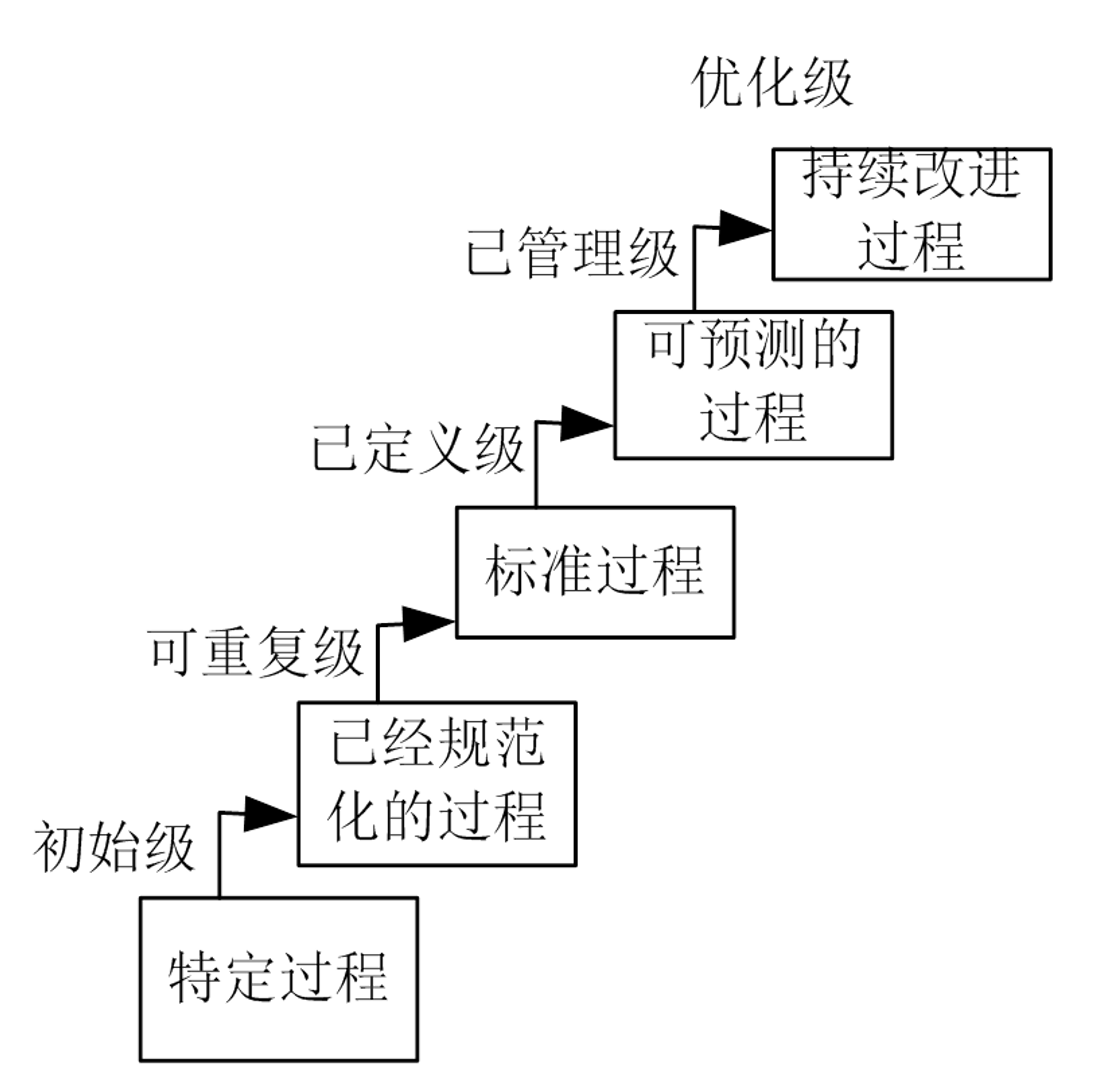
\includegraphics[width=\linewidth]{images/CMM1.png}
	\end{minipage}
	}
	\subfloat{
	\begin{minipage}[t]{0.56\linewidth}
	\centering
	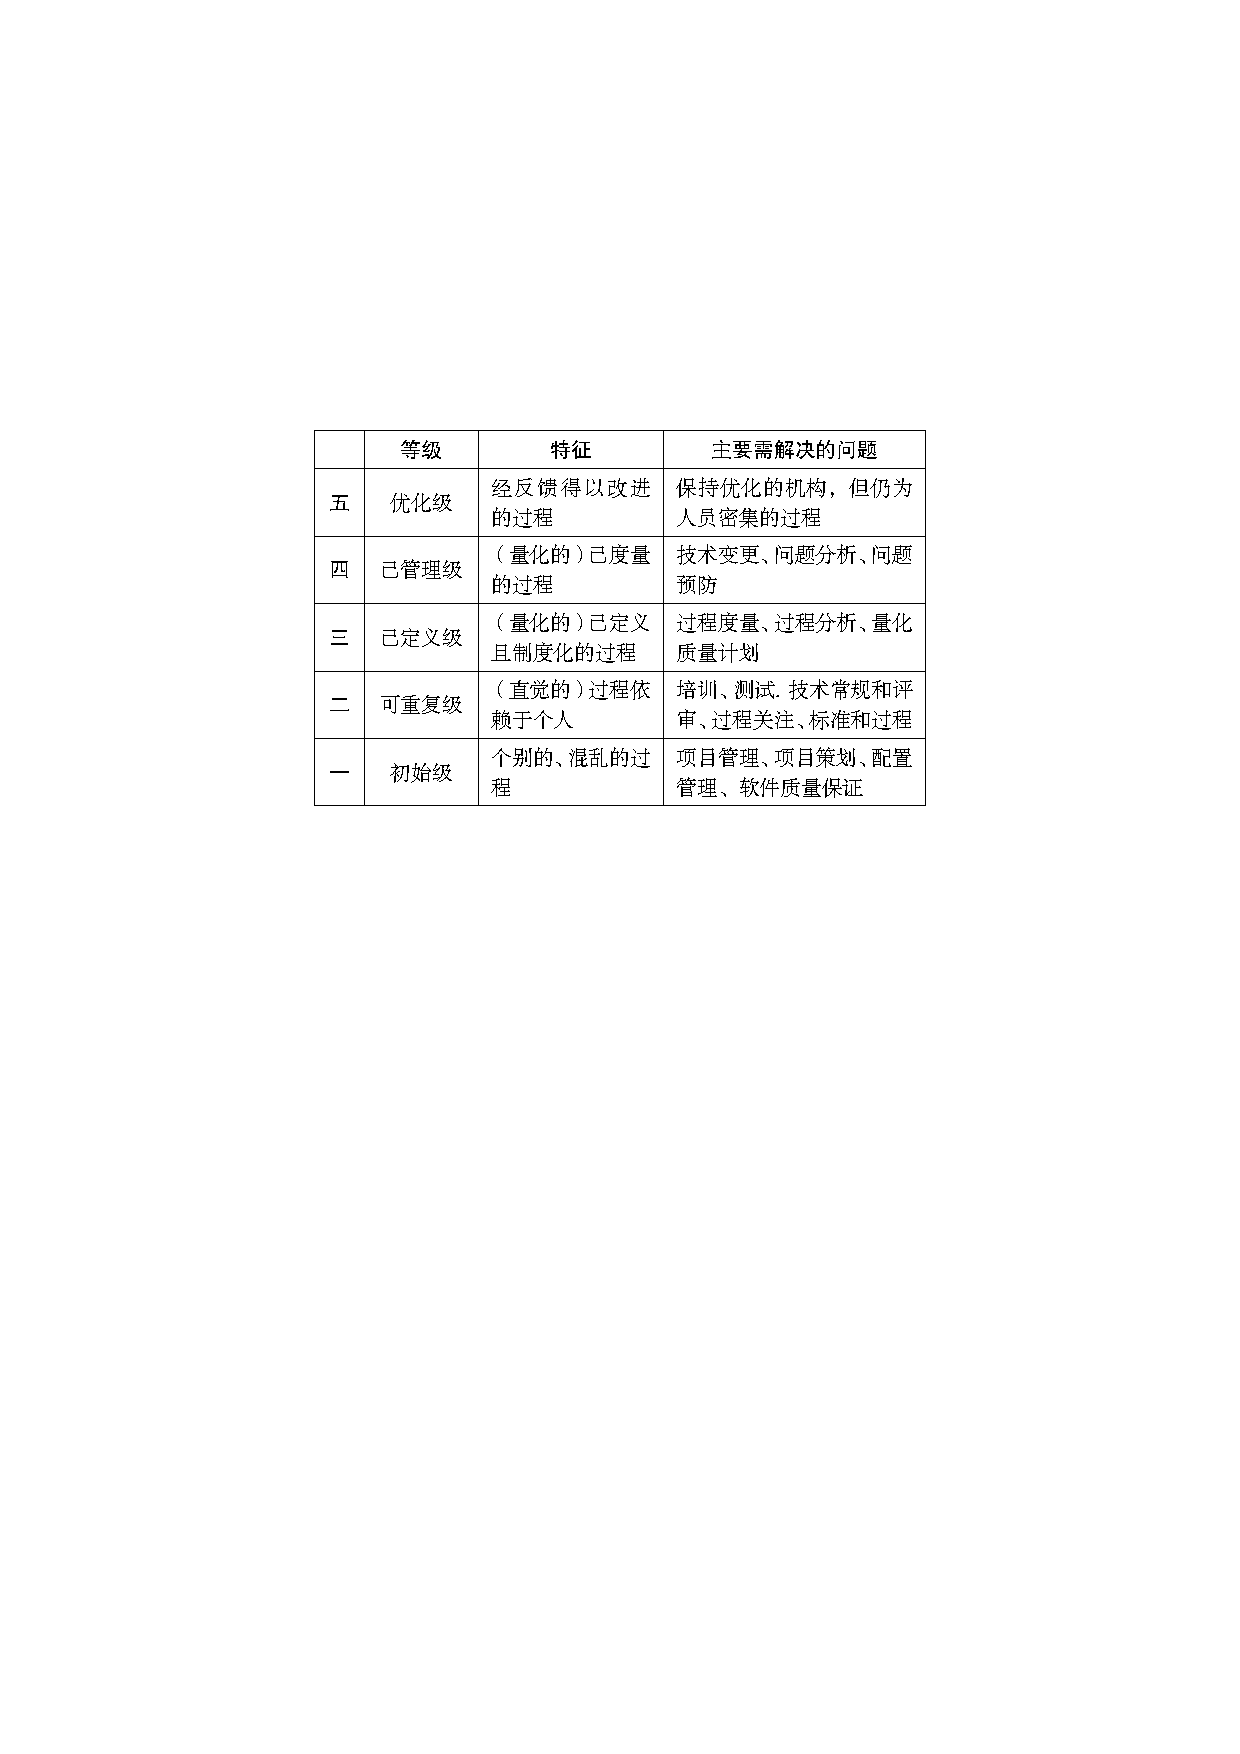
\includegraphics[width=\linewidth]{images/CMM2.pdf}
	\end{minipage}
	}
	\centering
\end{figure}


\subsubsection{考试题目}
\begin{problem}
	CMM的创始人是哪位?
	\uline{C}    
    \vspace{-0.8em}
    \begin{multicols}{4}
        \begin{enumerate}[label=\Alph*.]
            \item Boehm
            \item Juran
            \item Humphrey
            \item Crosby
        \end{enumerate}
    \end{multicols}
    \vspace{-1em}
\end{problem}


\subsection{软件过程管理/改进模型:CMMI}
CMMI (Capability Maturity Model Integration)能力成熟度集成模型
\begin{itemize}
    \item 刻画了软件团队/组织从不成熟到成熟的每个阶段的特征(也就是roadmap)
    \item 等级2和等级3关注的是当前状态
    \item 等级4和等级5是根据结果(未来)来进行管理
\end{itemize}

\subsubsection{等级一:初始级}
开发相对混乱,依赖个人英雄主义,没有过程概念,救火文化盛行
\begin{itemize}
    \item 软件组织对项目的目标与要做的努力很清晰,项目的目标可以实现
    \item 由于任务的完成带有很大的偶然性,软件组织无法保证在实施同类项目时仍然能够完成任务,项目实施是否成功主要取决于实施人员
\end{itemize}

\subsubsection{等级二:已管理级}
项目小组体现出项目管理的特征,有项目计划和跟踪、需求管理、配置管理等
\begin{itemize}
    \item 软件组织对项目有一系列管理程序,避免了软件组织完成任务的随机性,保证了软件组织实施项目的成功率
    \item 软件组织在项目实施上能够遵守既定的计划与流程,有资源准备,权责到人,对项目相关的实施人员进行相应的培训,对整个流程进行监测与控制,并联合上级单位对项目与流程进行审查
    \item 从2级升级到3级的原因:固化最佳实践,对小组而言是能够更快地学习其他的做法
\end{itemize}

\subsubsection{等级三:已定义级}
公司层面有标准流程和相应的规范,每个项目小组可以基于此定义自己的过程,使得优秀的做法可以在公司内分享
\begin{itemize}
    \item 软件组织能够根据自己的特殊情况及自己的标准流程,将这套管理体系与流程予以制度化
    \item 软件组织不仅能够在同类项目上成功,也可以在其他项目上成功
    \item 科学管理成为软件组织的一种文化,成为软件组织的财富
\end{itemize}

\subsubsection{等级四:定量管理级}
构建预测模型,以统计过程控制的手段来管理过程
\begin{itemize}
    \item 软件组织的项目管理实现了数字化
    \item 通过数字化技术来实现流程的稳定性,实现管理的精度,降低项目实施在质量上的波动
    \item 在这个级别我们希望能够看到一个预测模型
\end{itemize}

\subsubsection{等级五:优化级}
继续应用统计方法识别过程偏差,找到问题根源并消除,避免未来继续发生类似问题
\begin{itemize}
    \item 软件组织能够充分利用信息资料,对软件项目在项目实施的过程中可能出现的次品予以预防
    \item 能够主动地改善流程,运用新技术,实现流程的优化
\end{itemize}

\subsubsection{一些理解}
CMM/CMMI不适用于软件开发的原因
\begin{itemize}
    \item CMM/CMMI并不是一种具体的软件过程或者软件开发方法
    \begin{itemize}
        \item CMM/CMMI建立了一组有效地描述成熟软件组织特征的准则
        \item CMMI是过程改进模型而非软件过程或者软件过程模型:CMMI指导软件过程改进,不指导开发
        \item 按照CMM/CMMI模型的要求,一个软件组织应当定义使用本软件组织特点的软件过程,并且不断优化该过程,来更好地实现软件组织的商业目标
    \end{itemize}
    \item CMM/CMMI并不能作为检验软件过程优劣的标准:过程改进对不同企业的含义不一样,成熟度等级无法脱离企业环境直接横向比较
    \item CMM/CMMI与其他软件过程或者软件开发方法的比较是没有任何意义的
\end{itemize}

一些误解:
\begin{itemize}
    \item CMMI模型需要适当裁剪以适应公司的实际情况:需要裁剪的是公司内部定义的组织级开发流程和开发规范
    \item CMMI模型太重了,不适合互联网时代的轻量级开发:这个说法的错误之处在于,不一定是CMMI重或者轻,而是,CMMI根本就不是开发模型
    \item CMMI模型只适合大公司、大项目,不适合小项目:首先没人检验过;其次,项目的大小衡量本身也缺乏值得信赖的参考依据;最后,接受这种说法的人还是把CMMI当成是一种特殊的开发模型
    \item CMMI模型只适合需求不变或者很少变化的场合,不适合需求不确定,变化很多的场合:CMMI不是开发模型,与需求变化与否无关,谈不上适应或者不适应
\end{itemize}

{\kaishu CMMI不是过程优劣的标准,也不适合用作公司之间的能力比较:}正确,CMMI本身是有评级。(美国国防部订单招标要求企业至少达到CMMI的3级)。因为公司的能力需要绝对东西,也就是能力强,能力弱,而CMMI衡量的是相对的水平,CMMI仅仅关注在本公司的目标下的等级

更多讨论:试论CMM/CMMI不适合在当前软件开发当中应用的原因(\url{https://www.jianshu.com/p/b7407257eedb})

\subsubsection{考试题目}
\begin{problem}
请描述CMMI模型的5个等级的特征,并且解释为何CMMI模型不应该是敏捷方法的对立面。

五个等级的特征:
\begin{enumerate}[label=\arabic*.]
    \item Initial 原始级别:开发相对混乱,依赖个人英雄主义,没有过程概念,救火文化盛行
    \item Managed 已管理级别:项目小组体现出项目管理的特征,有项目计划和跟踪、需求管理、配置管理等
    \item Defined 已定义级别:公司层面有标准流程和相应的规范,每个项目小组可以基于此定义自己的过程,使得优秀的做法可以在公司共享。
    \item Quantitatively Managed 定量管理级别:构建预测模型,以统计过程控制的手段来管理过程
    \item Optimizing 优化级:继续应用统计方法识别过程偏差,找到问题根源并消除,避免未来继续发生类似问题
\end{enumerate}

原因解释:CMMI是过程管理/改进模型,刻画了软件组织从不成熟到成熟的路线图,而大部分敏捷方法都是开发方法,因此两者是完全不同性质的事物,将两者对立是不合适的

\begin{figure}[H]
    \vspace{-0.5em}
	\centering
	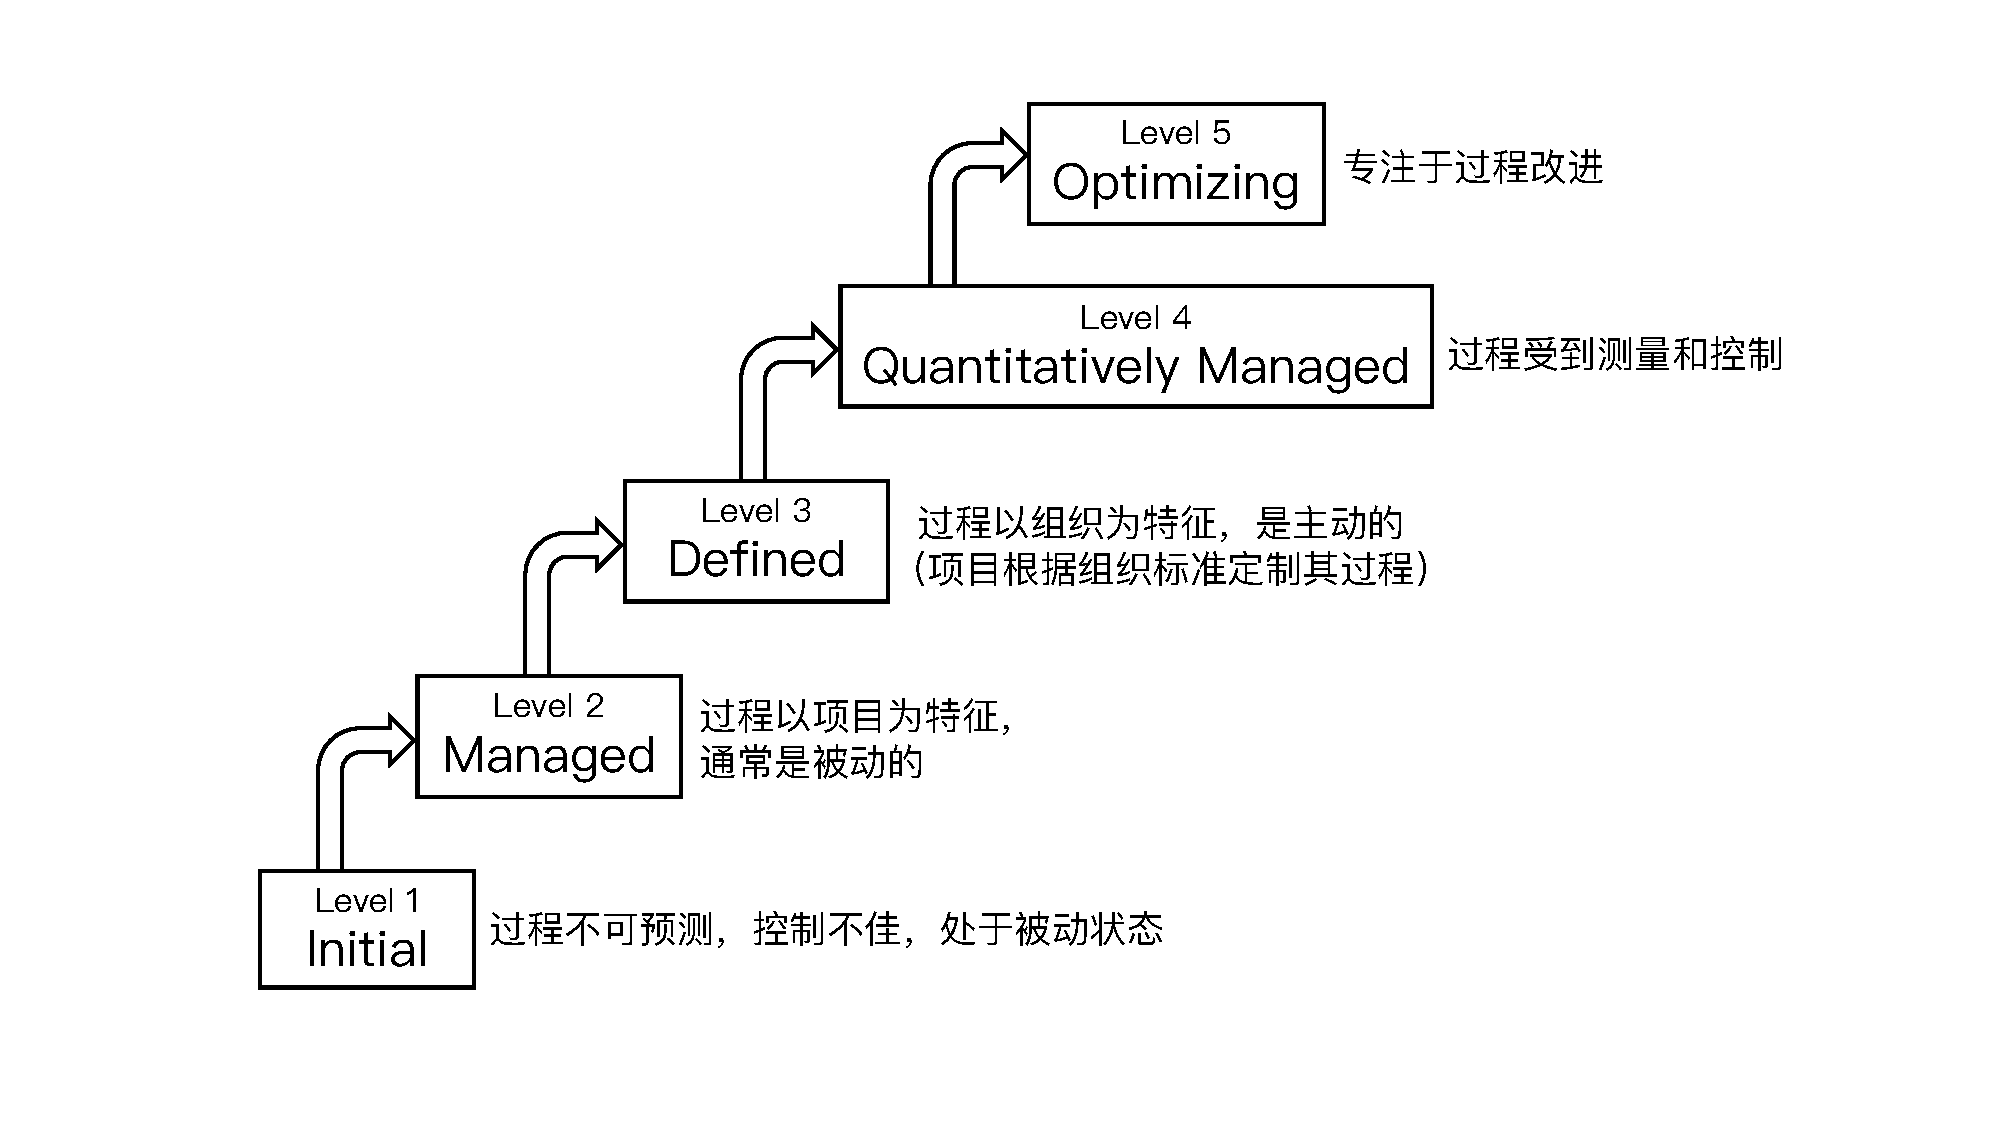
\includegraphics[width=0.65\textwidth]{images/CMMI.pdf}
    \vspace{-1em}
\end{figure}

\end{problem}


\subsection{软件过程改进模型:PDCA模型}
\begin{wraptable}{r}{6cm}
    \vspace{-4.5em}
	\centering
	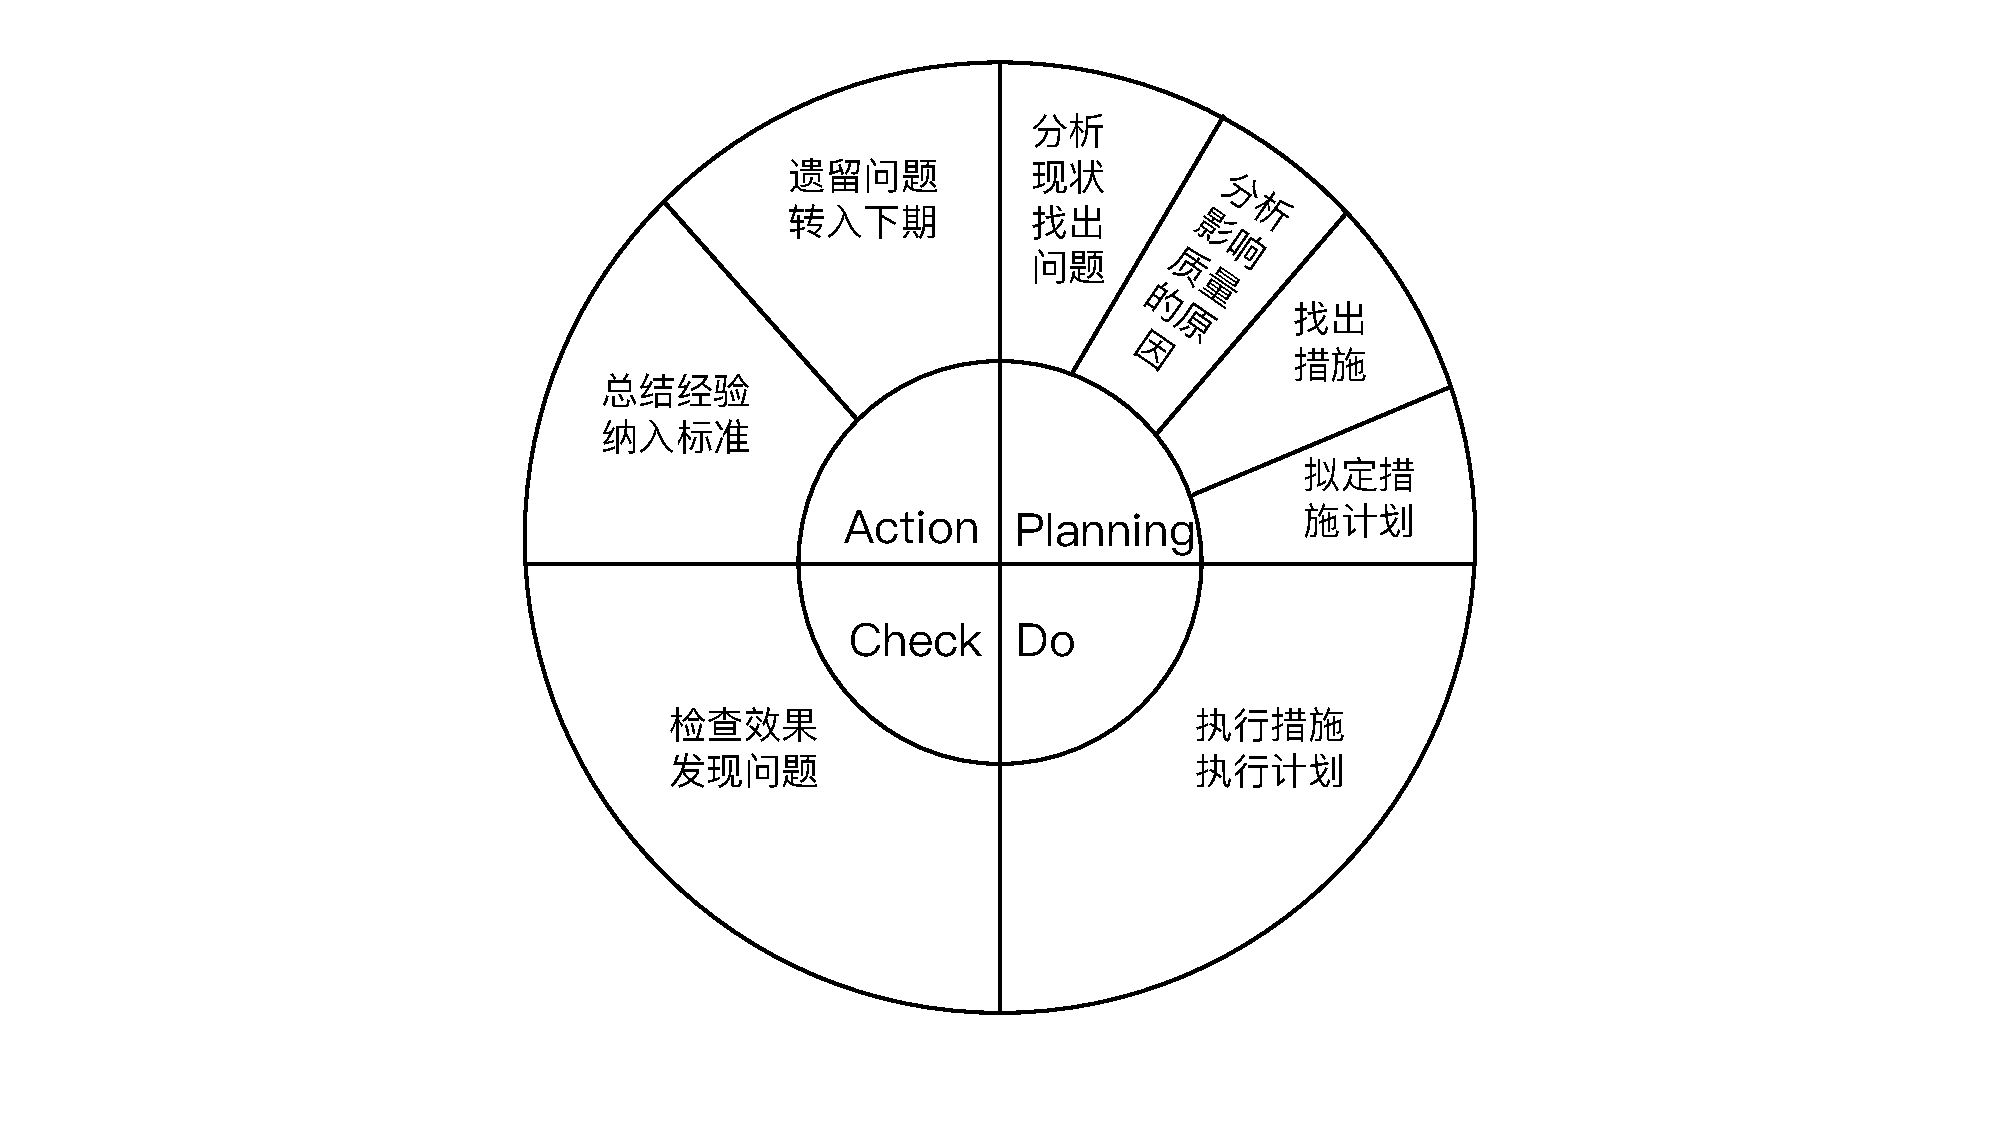
\includegraphics[width=0.4\textwidth]{images/PDCA.pdf}
    \vspace{-1em}
\end{wraptable}
PDCA模型的步骤:
\vspace{-0.8em}
\begin{multicols}{2}
    \begin{enumerate}[label=\arabic*.]
        \item 分析现状,找出问题
        \item 分析影响质量的原因
        \item 找出措施
        \item 拟定措施计划
        \item 执行措施,执行计划
        \item 检查效果,发现问题
        \item 总结经验,纳入标准
        \item 遗留问题转入下期PDCA循环
    \end{enumerate}
\end{multicols}
\vspace{-1em}

\subsubsection{考试题目}
\begin{problem}
请描述PDCA模型的主要步骤。
\end{problem}


\subsection{软件过程改进模型:IDEAL模型}
IDEAL模型解决了软件组织在各种质量改进环境下的需要。它包括了软件过程改进周期中的五个阶段,IDEAL是代表这五个阶段的单词的首字母
\vspace{-0.8em}
\begin{multicols}{3}
    \begin{itemize}
        \item I: Initiating 初始
        \item D: Diagnosing 诊断
        \item E: Establishing 建立
        \item A: Acting 执行
        \item L: Leveraging 调整
    \end{itemize}
\end{multicols}
\vspace{-1em}

\begin{figure}[H]
    \vspace{-0.5em}
	\centering
	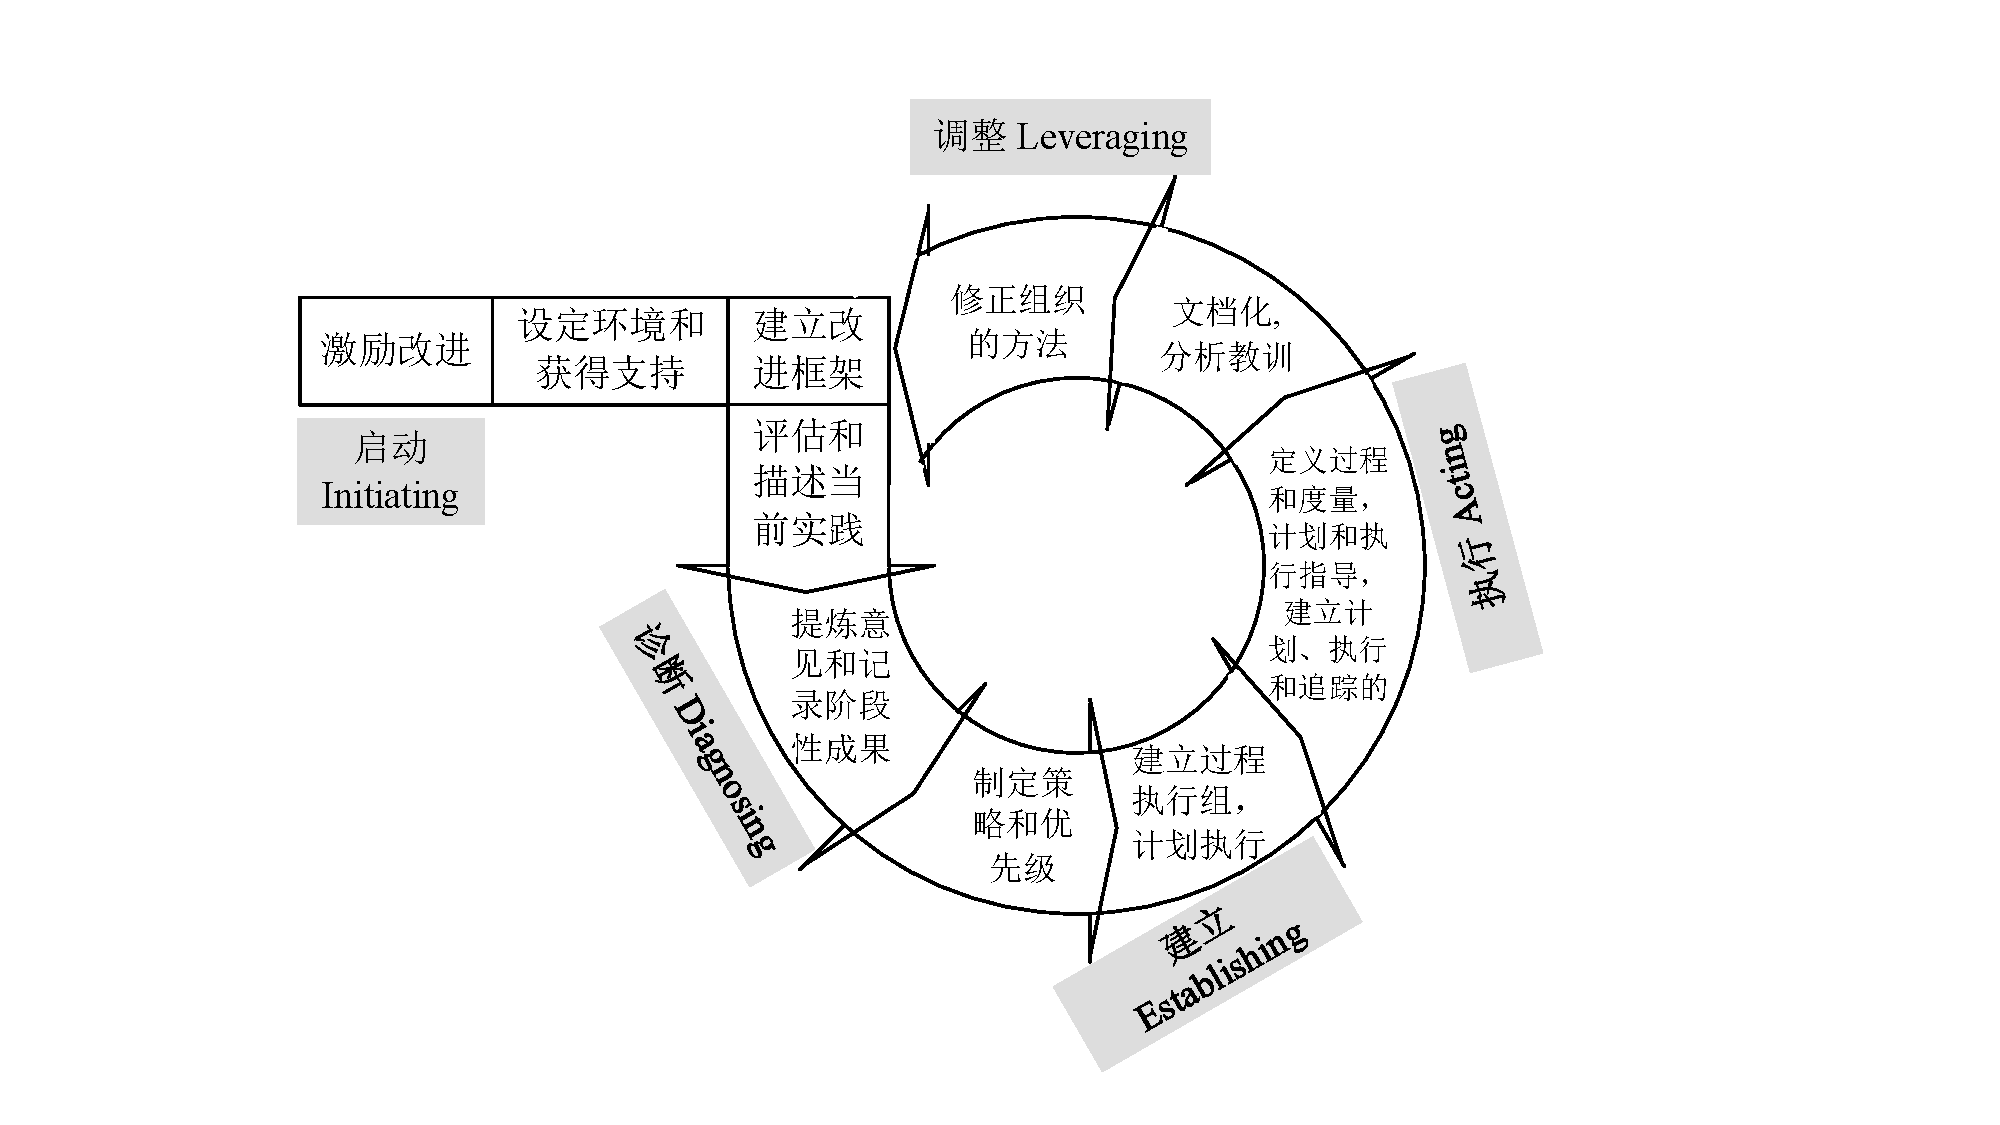
\includegraphics[width=0.63\textwidth]{images/IDEAL.pdf}
    \vspace{-1em}
\end{figure}


\subsection{软件过程管理模型:ISO/IEC 1504}
也叫SPICE (Software Process Improvement and Capability Determination),过程类别共有五种,分别是:
\vspace{-0.8em}
\begin{multicols}{3}
    \begin{itemize}
        \item 客户-供应商(CUS)过程
        \item 工程(ENG)过程
        \item 支持(SUP)过程
        \item 管理(MAN)过程
        \item 组织(ORG)过程
    \end{itemize}
\end{multicols}
\vspace{-1em}

重点关注“过程质量”,强调“持续改进”,获得ISO 9000标准认证的企业应该具有CMM第$2\sim 3$级的水平


\subsection{软件过程框架:RUP}
Rational统一过程(Rational Unified Process, RUP),它是由Rational软件公司推出的一种软件过程

RUP总结了经过多年商业化验证的6条最有效的软件开发经验,这些经验被称为“最佳实践”
\vspace{-0.8em}
\begin{multicols}{3}
    \begin{enumerate}[label=\arabic*.]
        \item 迭代式开发
        \item 管理需求
        \item 使用基于构件的体系结构
        \item 可视化建模
        \item 验证软件质量
        \item 控制软件变更
    \end{enumerate}
\end{multicols}
\vspace{-1em}

RUP软件开发生命周期:
\begin{enumerate}[label=\arabic*.]
    \item 初始阶段:建立业务模型,定义最终产品视图,并且确定项目的范围
    \item 精化阶段:设计并确定系统的体系结构,制定项目计划,确定资源需
    \item 构建阶段:开发出所有构件和应用程序,把它们集成为客户需要的产品,并且详尽地测试所有功能
    \item 移交阶段:把开发的产品提交给用户使用
\end{enumerate}

\subsection{软件质量管理发展}
\begin{problem}
描述下述质量管理大师的主要观点和贡献,工作对软件过程和项目管理的借鉴意义
\end{problem}

\subsubsection{Shewhart}
\begin{itemize}
    \item 最早将\textbf{统计控制}的思想引入质量管理,是质量改进奠基人
    \item 提出PDS模型(计划执行检查Plan-Do-See),后被戴明进一步发展为PDCA
\end{itemize}

\subsubsection{Deming}
\begin{itemize}
    \item \textbf{质量改进}:提出质量改进的思想,被称为日本质量管理之父
    \item \textbf{PDCA循环}:提出PDCA循环,被称为“\textbf{戴明环}”(Plan、Do、Check、Action),为最基本的质量和管理工具
\end{itemize}

\textbf{戴明管理14条原则:}
\vspace{-0.8em}
\begin{multicols}{2}
    \begin{enumerate}[label=\arabic*.]
        \item 树立改进产品和服务的坚定目标
        \item 采用新的思维方法
        \item 停止依赖检验的办法获得质量
        \item 不再凭价格标签进货
        \item 坚持不懈地提高产品质量和生产率
        \item 岗位培训制度化
        \item 管理者的作用应突出强调
        \item 排除畏难情绪
        \item 打破部门和人员之间的障碍
        \item 不再给操作人员提空洞的口号
        \item 取消对操作人员规定的工作定额和指标
        \item 不再采用按年度对人员工件进行评估
        \item 创建积极的自我提高计划制度
        \item 让每个员工都投入到提高产品质量的活动中去
    \end{enumerate}
\end{multicols}
\vspace{-1em}

\subsubsection{Juran}
\begin{itemize}
    \item 主编\textbf{质量控制手册}:《质量控制手册》为当今世界质量控制科学的“圣经”,奠定了“全面质量管理”TQM的理论基础(Total Quality Management)
    \item 提出\textbf{适用性质量}:
    \begin{itemize}
        \item 适用性质量:质量是一种适用性,即产品在使用期间能满足使用者的要求
        \item 质量不仅仅要满足明确的需求,还要满足潜在的需求。该思想使得质量管理范围从生产过程中的控制进一步扩大到产品开发和工艺设计阶段,即挖掘用户潜在需求
    \end{itemize}
    \item 提出\textbf{质量三步曲}:就是质量计划$\rightarrow$质量控制$\rightarrow$质量改进
    \item 提出\textbf{Juran质量螺旋}
    \item 提出\textbf{80/20原则}:认为有80\%的质量问题是由领导责任引起的,从而将人力与质量管理结合起来
\end{itemize}

\subsubsection{Crosby}
\begin{itemize}
    \item 提出\textbf{零缺陷}的概念:
    \begin{itemize}
        \item 零缺陷:第一次就把事情做对。想要做到这一点,就需要把工作放在预防上而不是质量检验上
    \end{itemize}
    \item 提出\textbf{质量管理}的绝对性:
    \vspace{-0.8em}
    \begin{multicols}{2}
        \begin{itemize}
            \item 质量就是符合要求,而不是“完美”
            \item 质量来自于预防,而不是检验
            \item 质量的标准是“零缺陷”,而不是可接受质量水平
            \item 质量的衡量标准是“不符合要求的代价”
        \end{itemize}
    \end{multicols}
    \vspace{-1em}
    \item 提出质量改进的基本要素(6C-变革管理的六个阶段):
    \vspace{-0.8em}
    \begin{multicols}{2}
        \begin{itemize}
            \item 领悟(Comprehension):理解质量真谛
            \item 承诺(commitment):制定质量策略的决心
            \item 能力(capability):教育与培训
            \item 沟通(communication):成功的经验文档化、制度化
            \item 改正(correction):预防与提高绩效
            \item 坚持(continuance):强调质量管理成为一种工作方式
        \end{itemize}
    \end{multicols}
    \vspace{-1em}
    \item 发展质量成熟度的度量
\end{itemize}


\subsubsection{Humphrey 软件过程之父}
\begin{itemize}
    \item 采用Crosby的成熟度度量,提出了软件能力成熟度模型(CMM) ,对于软件过程管理与改进具有建设性作用
    \item 将上述的理论和实践引入软件过程
\end{itemize}

